%!TEX root = ./Basilisk-SPACECRAFTPLUS-20170808.tex

\section{Progress Explanation and Current Status}

This module is IN PROGRESS and this section lists the current progress and status of the module as capability is added to the module this document needs to be updated. This document should always be describing the current status of the module. 

Below is a list describing the limitations and status of the module

\begin{itemize}
	\item The first major status that needs to be understood is that the HingedRigidBody stateEffector is the only stateEffector at this time that is ready to be used with the multi-spacecraft architecture. The reason that each stateEffector needs to be updated is because it was found with stateEffectors that have multiple degrees of freedom change the generalized interaction between spacecraftDynamics and the individual stateEffectors. However, this change is relatively small to each stateEffector as long as the developer understands the steps to make the change. The architecture is proven to work with hingedRigidBodies and each stateEffector just needs to follow suit. 
	
	So in other words, if a stateEffector wants the capability of being able to be simulated in the mult-spacecraft environment some modifications need to be implemented to the specific stateEffectors. The hingedRigidBody stateEffector acts as a detailed example on the method to convert a stateEffector to allow for the mult-spacecraft interaction. Below is a further on how to implement this change:
	\begin{itemize}
		\item The prependSpacecraftNameToStates() method needs to be implemented for the corresponding stateEffector states just like hingedRigidBody does for its states. This allows for the stateEffector to know about the individual spacecraft that it is attached to.
		\item The linkInStates method needs to prepend the linked states from the spacecraft it is attached to, to get the corresponding state from the spacecraft. However, it should be noted that you can see the hingedRigidBody no longer needs access to the hubs primary state variables. This is because the backSubstitution methods now provide the stateEffectors with the appropriate Hub states in the method calls. Therefore there is not a need for stateEffectors to link to any of the Hubs state variables.
		\item The last step is to provide the contributions from the stateEffectors about point $P$ and frame $\cal P$. Again, this cannot be generalized because of multiple degree of freedom effectors so each effector has the job of being provide their contributions about point $P$ and frame $\cal P$. It should be noted that if the spacecraft is independent then point $B$ will be coincident with point $P$ and dcmPB will be identity. Therefore the math should work for both connected and unconnected spacecraft. Let me explain this in more detail with the hingedRigidBody:
		
		You can see that in the private variables in hingedRigidBody, that the variables have been changed to be point $P$ and $\cal P$ relative. Again, if single spacecraft is being implemented then frames $\cal B$ and $\cal P$ are coincident. In the stateEffector.h it shows that each stateEffector has access to these two crucial variables: r\_BP\_P and dcm\_BP. r\_BP\_P is defaulted to zero and dcm\_BP is defaulted to identity. With that knowledge, each stateEffector needs to use those variables and defined their contributions about about point $P$ and frame $\cal P$. about point $P$ and frame $\cal P$. The easiest way to implement this correctly, is to to change any internal variables (hopefully they are already indicated as private variables) to point $P$ and frame $\cal P$ relative. Therefore, values being set by python shouldn't be changed, but internal variables or intermediate variables should be changed. 
		\item Once a model has been changed to allow for multi spacecraft, it can be tested by using the test\_multi-spacecraft and add the stateEffector to the spacecraft system just like hingedRigidBodies are. If energy and momentum is conserved the stateEffector most likely was changed correctly. Obviously all other tests should pass.
	\end{itemize}

The following table describes the current status of each stateEffector being implemented in the multi-spacecraft environment. This table should be updated as stateEffectors have this added capability. 

\begin{table}[htbp]
	\caption{Test results.}
	\label{tab:results}
	\centering \fontsize{10}{10}\selectfont
	\begin{tabular}{c | c | c } % Column formatting, 
		\hline
		\textbf{Test} 				    & \textbf{Pass/Fail} &  \\ \hline
		HingedRigidBodies  & \textcolor{ForestGreen}{Implemented} & \textcolor{ForestGreen}{Tested} \\
		LinearSpringMassDamper  & \textcolor{Red}{Not Implemented} & \textcolor{Red}{Not Tested} \\ 
		SphericalPendulum  & \textcolor{Red}{Not Implemented} & \textcolor{Red}{Not Tested} \\ 
		FuelTank  & \textcolor{Red}{Not Implemented} & \textcolor{Red}{Not Tested} \\ 
		VSCMGs  & \textcolor{Red}{Not Implemented} & \textcolor{Red}{Not Tested} \\ 
		dualHingedRigidBodies  & \textcolor{Red}{Not Implemented} & \textcolor{Red}{Not Tested} \\ 
		nHingedRigidBodies  & \textcolor{Red}{Not Implemented} & \textcolor{Red}{Not Tested} \\ 
		\hline
	\end{tabular}
\end{table}
\clearpage

\item DynamicsEffectors need the same point $P$ and frame $\cal P$ relative math to be implemented. This would be done very similar to the hingedRigidBody effectors and once it has been implemented for the stateEffectors the jump to dynamicEffector is small. But as such a current progress table is shown below:

\begin{table}[htbp]
	\caption{Test results.}
	\label{tab:results}
	\centering \fontsize{10}{10}\selectfont
	\begin{tabular}{c | c | c } % Column formatting, 
		\hline
		\textbf{Test} 				    & \textbf{Pass/Fail} &  \\ \hline
		Thrusters  & \textcolor{Red}{Not Implemented} & \textcolor{Red}{Not Tested} \\ 
		ExtForceTorque  & \textcolor{Red}{Not Implemented} & \textcolor{Red}{Not Tested} \\ 
		ExtPulsedForceTorque  & \textcolor{Red}{Not Implemented} & \textcolor{Red}{Not Tested} \\ 
		dragEffector  & \textcolor{Red}{Not Implemented} & \textcolor{Red}{Not Tested} \\ 
		radiationPressure  & \textcolor{Red}{Not Implemented} & \textcolor{Red}{Not Tested} \\ 
		\hline
	\end{tabular}
\end{table}

\item On further evaluation, there is a bug believed to be in spacecraftDynamics with the multi-connected hubs. The attached hubEffectors needs to provide their contribution to the primary spacecraft about point $P$ and $\cal P$. Just like the other stateEffectors the hubEffector needs to be changed. This should be a small change, but nees to be done! The tests in this document do not show this bug because the contributions are not being added in spacecraftDynamics. So to be clear there is a bug in both spacecraftDynamics (because the attached hubs are not being looped over) and in the hubEffector (not providing contributions about point $P$ and $\cal P$) This is BUG that needs to be fixed.
 
\item The docking and detachment of spacecraft needs to be implemented in the spacecraftDynamics class. Currently the docking and detaching could be done using python (by stopping the sim at a specific time step and dock/detach from python) but this is not the intended use of this multi-spacecraft architecture. This NEEDS to be implemented in the spacecraftDynamics class that would allow for a message to be written out to the system which would allow for detachment and docking of the spacecraft. The kinematics of the docking locations would need to be taken into account in this docking/detaching method. (DockingData is the struct that holds the docking information of each dock) However, once this method is added, the rest of architecture would allow for the docking and detaching to happen seamlessly. The docking and detaching method should be called at the end of the SpacecraftDynamics::integrateState method.

\item The interaction between sensors and environment models has yet to be tested for the multi-spacecraft architecture. 
 
\end{itemize}

\section{Model Description}

\subsection{Introduction}

A detailed descrtiption of this architecture can be seen in: http://hanspeterschaub.info/Papers/grads/CodyAllard.pdf. Figure~\ref{fig:FlexSloshFigure} shows a schematic of what this module is intended to to do: simulate multiple spacecraft at a time that can dock and detach throughout the simulation. 

\begin{figure}[htbp]
	\centerline{
		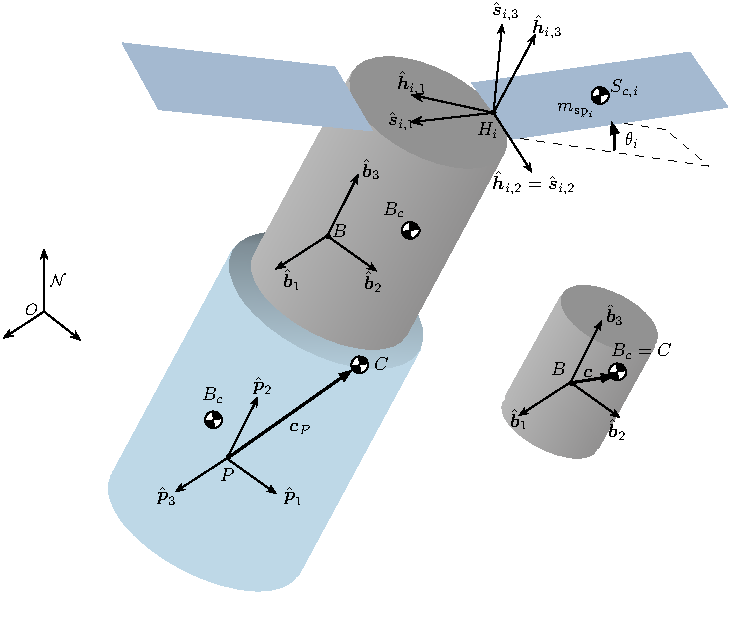
\includegraphics[width=0.8\textwidth]{Figures/multiSC}}
	\caption{Complex multi-spacecraft that can be simulated using spacecraftDynamics}
	\label{fig:FlexSloshFigure}
\end{figure}
